\documentclass[10pt,oneside,slovak,a4paper]{article}

\usepackage[slovak]{babel}
%\usepackage[T1]{fontenc}
\usepackage[IL2]{fontenc}
\usepackage[utf8]{inputenc}
\usepackage{graphicx}
\usepackage{url} % príkaz \url na formátovanie URL
\usepackage{hyperref} % odkazy v texte budú aktívne (pri niektorých triedach dokumentov spôsobuje posun textu)

\usepackage{cite}
%\usepackage{times}

%Nastavenie cesty pre obrazky
\graphicspath{ {./images/} }

\pagestyle{headings}

\title{Aplikácie a riešenia dištančného vzdelávania a e-vzdelávania\thanks{Semestrálny projekt v predmete Metódy inžinierskej práce, ak. rok 2020/21, vedenie: Ing. Fedor Lehocki, PhD.}}

\author{Lukáš Štrbo\\[2pt]
	{\small Slovenská technická univerzita v Bratislave}\\
	{\small Fakulta informatiky a informačných technológií}\\
	{\small \texttt{xstrbol@stuba.sk}}
	}

\date{\small 2. október 2020}



\begin{document}

\maketitle

\begin{abstract}
E-vzdelávanie sa stáva stále viac populárnejšou metódou nadobúdania vedomostí. Mnohí ľudia ju preferujú najmä kvôli rýchlosti a efektívnosti získavania poznatkov.
Prostredníctvom internetu sa dokážeme vzdelávať pomocou rôznych aplikácií, webov, kurzov alebo aj diskusných fór.
S e-vzdelávaním ide ruka v ruke dištančné vzdelávanie, ktoré hlavne v ťažších časoch, ako je napríklad nemožnosť zúčastňovať sa prezenčnej výučby z dôvodu pandémie COVID-19, 
 je voľbou číslo jedna. Rozdiely v medzi e-vzdelávaním a dištančným vzdelávním si rozoberieme v kapitole \ref{rozdiely}. Cieľom tejto práce je sprehľadniť čitateľovi rôzne metódy dištančného vzdelávania. Rozoberieme si a porovnáme riešenia dištančného vzdelávania a ich priamu
 aplikáciu. Zameriame sa na výhody a nevýhody, ale aj ktoré softvéry alebo platformy sú lepšie pre dištančné vzdelávanie v praxi. 
 V rámci porovnávania sa zameriame aj na efektivitu a aplikáciu daných metód dištančného vzdelávania.
\end{abstract}



\section*{Úvod} %Nezobrazi sa cislovanie
\label{uvod}
%Uvod do problematiky
Vzdelávanie sa prostredníctvom počítača a webu sa stáva stále viac populárnejšou a častejšou metódou výučby či sa jedná o školy alebo o samoukov. V súvislosti aj s celosvetovou pandémiou 
 COVID-19 bola väčšina škôl nútená prejsť na dištančné vzdelávanie. Pod dištančným vzdelávaním rozuemieme aj e-learning. Tieto výrazy si rozoberieme v kapitole\ref{rozdiely}.  

\section{Definícia dištančného vzdelávania a e-vzdelávania}
\label{rozdiely}
\subsection{Dištančné vzdelávanie}
Dištančné vzdelávanie zvyčajne zahŕňa situáciu, kde sú študenti oddelení od učiteľov na diaľku. Dištančné vzdelávanie zahŕňa poskytovanie systémov (elektronických alebo iných) na nadviazanie a udržiavanie komunikácie medzi učiteľmi a študentmi. Využíva určitú formu pedagogickej výmeny  medzi učiteľom a študentom na podporu učenia a hodnotenia.
Stará koncepcia dištančného vzdelávania bola spojená výlučne s tlačenými materiálmi, zatiaľ čo nová koncepcia dištančného vzdelávania zahŕňa doplnkový materiál používaný prostredníctvom netlačených médií, ako je rozhlas, televízia, počítače, notebooky, nahrané prednášky vo formáte videí, prostredníctvom projektorov, videokonferencií a interaktívnych stretnutí medzi študentmi.
Existujú 2 typy dištančného vzdelávania na základe interakcie študentov a to synchrónne a asynchrónne. Synchrónna metóda vyžaduje účasť študenta tvárou v tvár. Interakcia sa uskutočňuje v „reálnom čase“ a je bezprostredná. Asynchrónna nevyžaduje žiadnu účasť. Potreba, aby sa študenti a učitelia zhromaždili na stretnutí, je vylúčená a študenti si sami zvolia vlastný časový rámec pre interakciu. \cite{India}
\subsection{E-vzdelávanie}
E-learning je prirodzene vhodný na dištančné a flexibilné vzdelávanie, ale dá sa použiť aj v spojení s výučbou tvárou v tvár. V takom prípade sa bežne používa termín Blended learning. E-learning môže tiež odkazovať na vzdelávacie webové stránky, ako napríklad webové stránky ponúkajúce pracovné listy a interaktívne cvičenia pre deti. Tento výraz sa široko používa aj v obchodnom sektore, kde sa všeobecne vzťahuje na nákladovo efektívne online školenie. E-Learning je využitie technológií na podporu a zlepšenie výučby. So zameraním na používanie internetu v e-vzdelávaní sa objavili tri hlavné spôsoby použitia. Jedná sa o elektronickú technológiu na poskytovanie, podporu a zdokonaľovanie výučby a učenia sa.\cite{elearningDef}

\section{Typy dištančnej výučby}
%Uvod do typov distancnej vyucby
Dištančnou výučbou rozumieme :
\begin{itemize}
	\item \textbf{Technology-based training (TBT)} alebo aj e-vzdelávenie\cite{WiktorzakKotowski}
	\item \label{CBT} \textbf{Computer-based trainig (CBT)} ktorý používa počítače vo výučbovom procese na prenos znalostí, vykonávanie cvičení alebo simulácii. V rámci tohto konceptu sú aj rôzne kurzy, kedysi dodávané na CD.\cite{WiktorzakKotowski}
	\item \label{WBT}\textbf{Web-based training (WBT)} je typ dištančnej výučby, ktorý prebieha na internete prostredníctvom protokola TCP/IP. Zahŕňa prenos znalostí ako aj ich overenie, komunikáciu medzi používateľmi a riadením vzdelávacieho procesu s využitím webových stránok a webových aplikácií.\cite{WiktorzakKotowski}
\end{itemize}
Vyššie spomenuté typy dištančnej výučby sú spojené s použítím špecifických technológií. 
Avšak najviac používaný edukačný model kombinuje počítačovú technológiu s tradičným spôsobom vedenia tried na univerzitách.\\ 
V dôsledku toho môžeme rozlíšiť dištančnú výučbu na :
\begin{itemize}
	\item \textbf{Instructor-led training (ILT)} je výučbový proces v ktorom učiteľ vyučuje skupinu študentov. Hodiny prebiehajú väčšinou priamo v priestoroch školy.
Tradičná výučba môže nadobudnúť aj takú formu počas ktorej učiteľ komunikuje so žiakmi prostredníctvom internetu.\cite{WiktorzakKotowski}
	\item \textbf{Synchronous learning (SL)} znamená, že aktivity a výučba sú vedené v reálnom čase ale sú realizované cez internet. \cite{WiktorzakKotowski}
	Študenti aj učitelia sú prihlásení do jedného systému, takzvaného "virtuálneho učebného priestoru.\cite{WiktorzakKotowski}
	\item \textbf{Blended learning (BL)} alebo aj hybridné vyučovanie je spôsob výučby, ktorý kombinuje tradičný model výučby s dištančnou formou výučby.
	V tomto modeli je obsah prednášok prednášaný väčšinou vzdialene a prebiehajú on-line konzultácie, zatiaľ čo cvičenia a praktické hodiny sa uskutočňujú na priamo univerzite prezenčnou formou.\cite{WiktorzakKotowski} 
\end{itemize}


\begin{figure}[h]
	\centering
	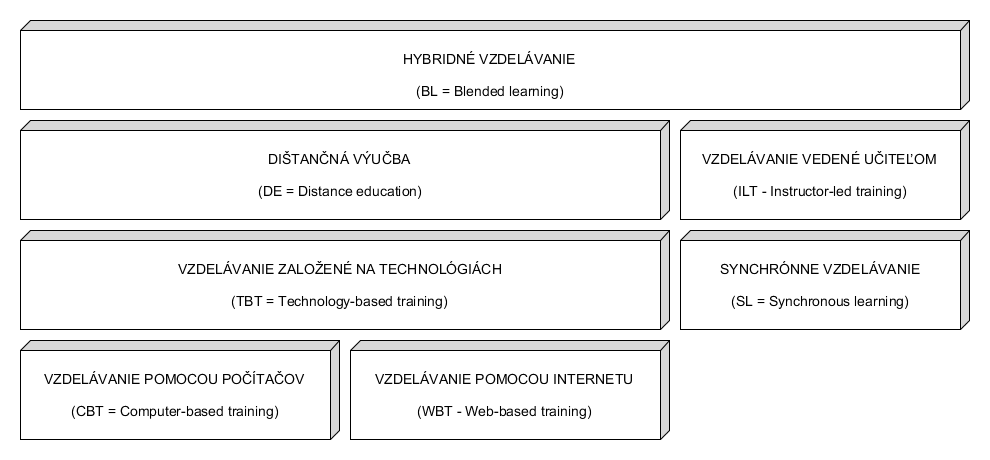
\includegraphics[width=\textwidth]{Vztahy_DE.png}
	\caption{Vzťahy medzi pojmami v dištančnom vzdelávaní\cite{WiktorzakKotowski}}
	\label{Vztahy_medzi_pojmami}
\end{figure}

%Referencia na obrazok
Vzťahy medzi pojmami spojenými s dištančným vzdelávaním sú znázornené na obrázku \ref{Vztahy_medzi_pojmami}.
Oblasť dištančného vzdelávania pokrýva širokú oblasť technológií a metód vzdelávania. 
Je to okrem iného spôsobené potrebou neustálej odbornej prípravy v čoraz viac oblastiach.
V závislosti od prenášaného obsahu (napr. kurz v angličtine), sa používajú rôzne nástroje a rôzne techniky výučby.\cite{WiktorzakKotowski}
%V nasledujúcej časti nájdete stručný popis nástrojov dištančného vzdelávania.

\section{Vývoj podporných systémov pre dištančné vzdelávanie}%ALEBO : Podporne systemy pre distancne vzdelavanie


\subsection{Komunikačné platformy}
%Webex, Meet, MS TEAMS, porovnanie , obluba u studentov, vlastnosti
\subsection{Edukačné platformy}
%Edukacne platformy - Online testovanie , Edupage, AIS, Kurzy online, Moodle, ...


\section{Výhody a nevýhody dištančnej výučby}
\subsection{Výhody}
\begin{itemize}
	\item Pre študovanie na diaľku študent potrebuje iba počítač, tablet alebo smartfón s prístupom na internet. Študent sa sám rozhodne, kedy a kde bude materiál študovať.\cite{Sokolova2018}
	\item Navyše, vďaka možnosti študovať na diaľku existuje možnosť, ako ušetriť peniaze na školenie, náklady na dopravu a tiež ubytovanie pre študentov v metropolitnej oblasti.
	Študenti nemusia platiť za učebnice, ďalšiu literatúru, neprenajímajú si dom ani nebývajú v internáte.\cite{Sokolova2018}
	\item Ďalšou z výhod je, že ak niektorí študenti niečo nepochopili, nie vždy sa odvážia položiť otázku lektorovi ale v rámci dištančného vzdelávania sa plachí študenti cítia pohodlnejšie.
	Študenti, ktorí potrebujú viac času na premýšľanie o informáciách ako ich spolužiaci, si zároveň môžu prednášku vypočuť viackrát, dlhšie sa zamýšľajú nad poskytnutým materiálom a potom, ak ešte niečo zostane nezrozumiteľné, opýtajú sa lektora.\cite{Sokolova2018}
	\item Dištančné vzdelávanie umožňuje učiteľom rýchlo získať spätnú väzbu od veľkého počtu študentov. Prebieha interaktívnou formou, takže je zamerané na dialóg.
	Lektor nie je iba „hovoriaca učebnica“. Každý študent má možnosť klásť lektorovi otázky, ktoré ho zaujímajú. Môže diskutovať ako so samotným lektorom, tak aj s ostatnými poslucháčmi.\cite{Sokolova2018}
	\item Ďalšou pozitívnou vlastnosťou dištančného vzdelávania je, že je ideálnou alternatívou denného štúdia pre ľudí so zdravotným postihnutím.
	Títo študenti musia na získanie vzdelania vynaložiť veľa fyzického, emocionálneho a finančného úsilia.
	Nie vždy majú možnosť fyzicky navštevovať hodiny kvôli zlému zdravotnému stavu alebo nutnosti podstúpiť ošetrenie v nemocnici.
	Niektorí z nich potrebujú špeciálne vybavené rampy pre invalidné vozíky, čo zase pred univerzitou predstavuje problém s vytváraním špeciálnych zariadení a zvyšuje náklady na údržbu a vybavenie priestorov.\cite{Sokolova2018} 
\end{itemize}
\subsection{Nevýhody}
\begin{itemize}
	\item Študent je zbavený živej komunikácie s lektorom aj s ostatnými študentmi.
	Prednáška, prednesená bez živej účasti príjemcov, stratí veľa na významovom obsahu a na emotívnom prednese, pretože nie každý lektor sa dokáže inšpirovať pohľadom na čiernu skrinku videokamery zameranú na neho počas natáčania, namiesto ľudské oči.\cite{Sokolova2018}
	\item Ďalším negatívnym aspektom dištančného vzdelávania je skutočnosť, že hanbliví študenti, ktorí sa cítia lepšie pri interakcii na diaľku, sa nikdy neprestanú báť vyjadrovať svoje myšlienky v prítomnosti iných ľudí na diaľku ale nezvyknú si na živú komunikáciu.\cite{Sokolova2018}
	\item Testovací systém je veľmi vhodný na diaľkové hodnotenie, ale nie je vhodný na rozvoj schopnosti samostatne myslieť, asimilovať materiál a snažiť sa ho nejako uplatniť vo svojom živote.
	Výsledky, ktoré získa študent po zvládnutí daného materiálu, preto nebudú vždy odrážať úroveň jeho vedomostí o otázkach a témach, ktoré študoval.\cite{Sokolova2018}
	\item Dlhodobé pracovanie na počítači má negatívny vplyv na zdravie, zrak, chrbticu.\cite{Sokolova2018}
\end{itemize}



\section{Aplikácia dištančnej výučby v praxi}
\subsection{Základné a stredné školy}
\subsection{Vysoké školy}
\subsection{Virtuálne univerzity}

\section{Efektivita a dopad dištančnej výučby}
\subsection{Efektívnosť}
\subsection{Výhody a nevýhody}


%\acknowledgement{Ak niekomu chcete poďakovať\ldots}



\bibliography{zdroje}
\bibliographystyle{plain}
\end{document}
